


\begin{figure}[hbt!]
    % \renewcommand{\arraystretch}{0.04}
    % \centering
    \Large
    \begin{tabular}{p{3.6cm}p{3.6cm}}
    \scalebox{0.495}{
    \hspace{-1.4cm}
        % This file was created with tikzplotlib v0.10.1.
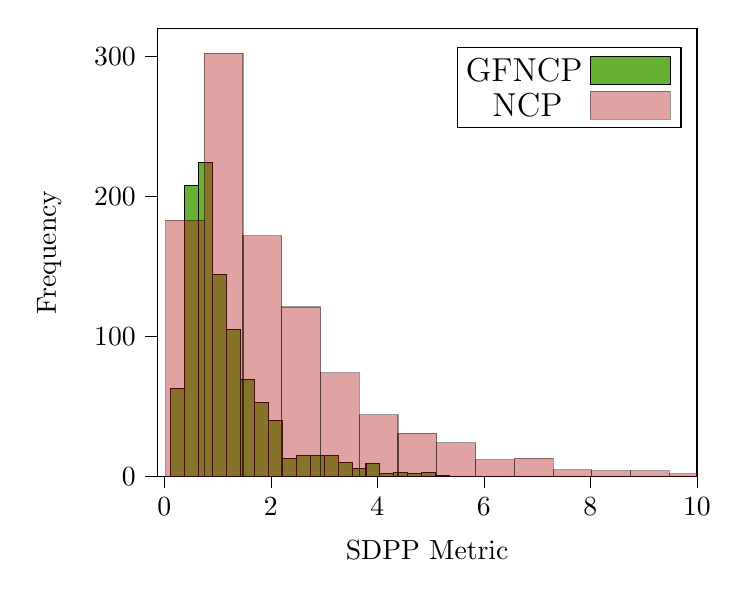
\begin{tikzpicture}

\definecolor{darkgray176}{RGB}{176,176,176}
\definecolor{green_1}{RGB}{173,216,230}
% \definecolor{green_1}{RGB}{173,216,230}
\definecolor{green_1}{rgb}{0.6, 0.81, 0.93}
\definecolor{forestgreen4416044}{RGB}{44,160,44}
\definecolor{red_1}{RGB}{178,24,24}
\definecolor{green_1}{rgb}{0.4, 0.69, 0.2}

\begin{axis}[
tick align=outside,
tick pos=left,
x grid style={darkgray176},
xlabel={SDPP Metric},
xmin=-0.13, xmax=10,
xtick style={color=black},
y grid style={darkgray176},
ylabel={Frequency},
ymin=0, ymax=320,
ytick style={color=black},
y label style={at={(axis description cs:-0.16,.5)},anchor=south},
x label style={at={(axis description cs:.5,-0.12)}},
]

\node[text width=1cm] at (6.4,290) {\large GFNCP};
\node[text width=1cm] at (6.9,265) {\large NCP};
\draw[draw=black,fill=green_1] (axis cs:8,280) rectangle (axis cs:9.5,300);
\draw[draw=black,fill=red_1,opacity=0.4] (axis cs:8,255) rectangle (axis cs:9.5,275);
\draw[draw=black,fill=green_1,fill opacity=0.0] (axis cs:5.5,249) rectangle (axis cs:9.7,306);

\draw[draw=black,fill=green_1] (axis cs:0.12332564212824,0) rectangle (axis cs:0.385047029624798,63);
\draw[draw=black,fill=green_1] (axis cs:0.385047029624798,0) rectangle (axis cs:0.646768417121357,208);
\draw[draw=black,fill=green_1] (axis cs:0.646768417121357,0) rectangle (axis cs:0.908489804617915,224);
\draw[draw=black,fill=green_1] (axis cs:0.908489804617915,0) rectangle (axis cs:1.17021119211447,144);
\draw[draw=black,fill=green_1] (axis cs:1.17021119211447,0) rectangle (axis cs:1.43193257961103,105);
\draw[draw=black,fill=green_1] (axis cs:1.43193257961103,0) rectangle (axis cs:1.69365396710759,69);
\draw[draw=black,fill=green_1] (axis cs:1.69365396710759,0) rectangle (axis cs:1.95537535460415,53);
\draw[draw=black,fill=green_1] (axis cs:1.95537535460415,0) rectangle (axis cs:2.21709674210071,40);
\draw[draw=black,fill=green_1] (axis cs:2.21709674210071,0) rectangle (axis cs:2.47881812959726,13);
\draw[draw=black,fill=green_1] (axis cs:2.47881812959726,0) rectangle (axis cs:2.74053951709382,15);
\draw[draw=black,fill=green_1] (axis cs:2.74053951709382,0) rectangle (axis cs:3.00226090459038,15);
\draw[draw=black,fill=green_1] (axis cs:3.00226090459038,0) rectangle (axis cs:3.26398229208694,15);
\draw[draw=black,fill=green_1] (axis cs:3.26398229208694,0) rectangle (axis cs:3.5257036795835,10);
\draw[draw=black,fill=green_1] (axis cs:3.5257036795835,0) rectangle (axis cs:3.78742506708005,6);
\draw[draw=black,fill=green_1] (axis cs:3.78742506708006,0) rectangle (axis cs:4.04914645457661,9);
\draw[draw=black,fill=green_1] (axis cs:4.04914645457661,0) rectangle (axis cs:4.31086784207317,2);
\draw[draw=black,fill=green_1] (axis cs:4.31086784207317,0) rectangle (axis cs:4.57258922956973,3);
\draw[draw=black,fill=green_1] (axis cs:4.57258922956973,0) rectangle (axis cs:4.83431061706629,2);
\draw[draw=black,fill=green_1] (axis cs:4.83431061706629,0) rectangle (axis cs:5.09603200456284,3);
\draw[draw=black,fill=green_1] (axis cs:5.09603200456284,0) rectangle (axis cs:5.3577533920594,1);

\draw[draw=black,fill=red_1,opacity=0.4] (axis cs:0.0244094305721065,0) rectangle (axis cs:0.751850527804012,183);
\draw[draw=black,fill=red_1,opacity=0.4] (axis cs:0.751850527804012,0) rectangle (axis cs:1.47929162503592,302);
\draw[draw=black,fill=red_1,opacity=0.4] (axis cs:1.47929162503592,0) rectangle (axis cs:2.20673272226782,172);
\draw[draw=black,fill=red_1,opacity=0.4] (axis cs:2.20673272226782,0) rectangle (axis cs:2.93417381949973,121);
\draw[draw=black,fill=red_1,opacity=0.4] (axis cs:2.93417381949973,0) rectangle (axis cs:3.66161491673163,74);
\draw[draw=black,fill=red_1,opacity=0.4] (axis cs:3.66161491673163,0) rectangle (axis cs:4.38905601396354,44);
\draw[draw=black,fill=red_1,opacity=0.4] (axis cs:4.38905601396354,0) rectangle (axis cs:5.11649711119544,31);
\draw[draw=black,fill=red_1,opacity=0.4] (axis cs:5.11649711119544,0) rectangle (axis cs:5.84393820842735,24);
\draw[draw=black,fill=red_1,opacity=0.4] (axis cs:5.84393820842735,0) rectangle (axis cs:6.57137930565925,12);
\draw[draw=black,fill=red_1,opacity=0.4] (axis cs:6.57137930565925,0) rectangle (axis cs:7.29882040289116,13);
\draw[draw=black,fill=red_1,opacity=0.4] (axis cs:7.29882040289116,0) rectangle (axis cs:8.02626150012306,5);
\draw[draw=black,fill=red_1,opacity=0.4] (axis cs:8.02626150012307,0) rectangle (axis cs:8.75370259735497,4);
\draw[draw=black,fill=red_1,opacity=0.4] (axis cs:8.75370259735497,0) rectangle (axis cs:9.48114369458687,4);
\draw[draw=black,fill=red_1,opacity=0.4] (axis cs:9.48114369458687,0) rectangle (axis cs:10.2085847918188,2);
\draw[draw=black,fill=red_1,opacity=0.4] (axis cs:10.2085847918188,0) rectangle (axis cs:10.9360258890507,5);
\draw[draw=black,fill=red_1,opacity=0.4] (axis cs:10.9360258890507,0) rectangle (axis cs:11.6634669862826,1);
\draw[draw=black,fill=red_1,opacity=0.4] (axis cs:11.6634669862826,0) rectangle (axis cs:12.3909080835145,1);
\draw[draw=black,fill=red_1,opacity=0.4] (axis cs:12.3909080835145,0) rectangle (axis cs:13.1183491807464,0);
\draw[draw=black,fill=red_1,opacity=0.4] (axis cs:13.1183491807464,0) rectangle (axis cs:13.8457902779783,1);
\draw[draw=black,fill=red_1,opacity=0.4] (axis cs:13.8457902779783,0) rectangle (axis cs:14.5732313752102,1);
\end{axis}

\end{tikzpicture}

    } & 
    \scalebox{0.495}{
        \hspace{-0.7cm}
        % This file was created with tikzplotlib v0.10.1.
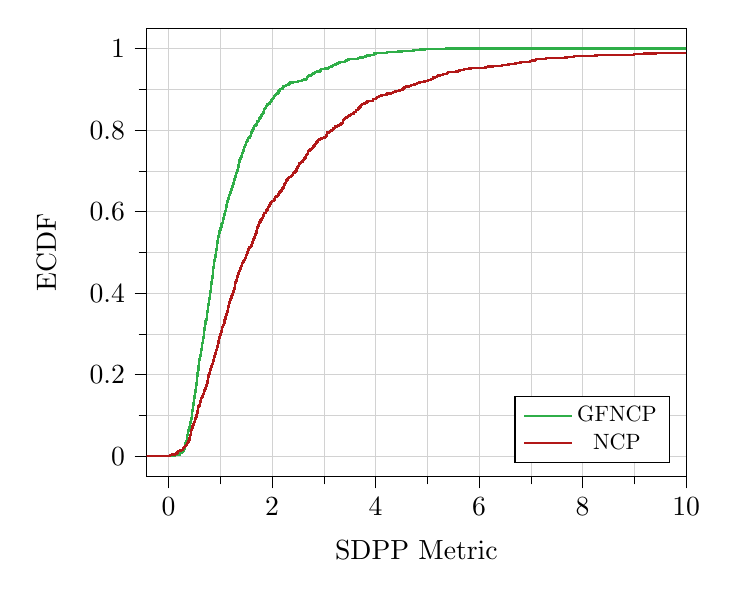
\begin{tikzpicture}

\definecolor{darkgray176}{RGB}{210,210,210}
\definecolor{steelblue31119180}{RGB}{31,119,180}
% \definecolor{darkgray176}{RGB}{176,176,176}
\definecolor{darkorange25512714}{RGB}{255,127,14}
\definecolor{forestgreen4416044}{RGB}{44,160,44}
\definecolor{steelblue31119180}{RGB}{31,119,180}
\definecolor{red_1}{RGB}{178,24,24}
\definecolor{green_1}{RGB}{47,174,72}


\begin{axis}[
tick align=outside,
tick pos=left,
x grid style={darkgray176},
xlabel={SDPP Metric},
xmin=-0.426289271614532, xmax=10,
xtick style={color=black},
y grid style={darkgray176},
ylabel={ECDF},
ymin=-0.05, ymax=1.05,
ytick style={color=black},
y label style={at={(axis description cs:-0.15,.5)},anchor=south},
x label style={at={(axis description cs:.5,-0.12)}},
legend pos=south east,
legend style={nodes={scale=0.8, transform shape}},
%
grid=both,
grid style={line width=.1pt, draw=gray!10},
major grid style={line width=.2pt,draw=gray!20},
minor x tick num=1,
minor y tick num=1,
%
]
\addlegendentry{GFNCP}
\addlegendentry{NCP}
\addplot [thick, green_1, const plot mark left]
table {%
-0.138395745368318 0
0.12332564212824 0.001
0.123975716273782 0.002
0.18867293646119 0.003
0.188836656892859 0.004
0.213405368424915 0.005
0.214643317844613 0.006
0.221498535618005 0.007
0.227032858043515 0.008
0.24118378829866 0.009
0.248816258941435 0.01
0.281617146566013 0.011
0.282163373363009 0.012
0.284585627167517 0.013
0.294463804314713 0.014
0.295347613115953 0.015
0.296696817637227 0.016
0.300329632591378 0.017
0.300948892186433 0.018
0.308818602390632 0.019
0.309030066575113 0.02
0.309874917138539 0.021
0.311081985245463 0.022
0.311325855387208 0.023
0.314660779642734 0.024
0.318334060115046 0.025
0.320522777826358 0.026
0.32111257670422 0.027
0.323468098702721 0.028
0.323988145944562 0.029
0.327874180122696 0.03
0.327938201051205 0.031
0.331287776207898 0.032
0.331823307071554 0.033
0.333218023534976 0.034
0.333815797102556 0.035
0.334722991131556 0.036
0.334841853477422 0.037
0.346921947214444 0.038
0.349585145053009 0.039
0.351464639459815 0.04
0.351761129544081 0.041
0.353542483354018 0.042
0.353611306948008 0.043
0.354030847918059 0.044
0.354314325394994 0.045
0.355473413591896 0.046
0.355880366342931 0.047
0.35878935063723 0.048
0.35972139729148 0.049
0.361654647943278 0.05
0.36313938856483 0.051
0.364550904892762 0.052
0.369946144839515 0.053
0.371121871622914 0.054
0.371128154728229 0.055
0.373800926356187 0.056
0.373870393287395 0.057
0.375556588242568 0.058
0.378946242954707 0.059
0.37951663176592 0.06
0.380810776778185 0.061
0.381644338698618 0.062
0.384806470918226 0.063
0.386256574909176 0.064
0.387491112320256 0.065
0.392960566625264 0.066
0.400968417229458 0.067
0.401563416722975 0.068
0.401667174185046 0.069
0.402587513692541 0.07
0.402966761782356 0.071
0.405843354354917 0.072
0.406897773596088 0.073
0.408671730937215 0.074
0.412242555334521 0.075
0.41247113337079 0.076
0.415098135729761 0.077
0.416022875755547 0.078
0.418591370810347 0.079
0.418772376792461 0.08
0.41882885099213 0.081
0.421102598261564 0.082
0.423077260249449 0.083
0.424858509302322 0.084
0.43243216787738 0.085
0.433119512654122 0.086
0.434346053173444 0.087
0.435819079631018 0.088
0.437149243051131 0.089
0.439080253670104 0.09
0.439392648980314 0.091
0.439530955853408 0.092
0.440626156013795 0.093
0.442922551780318 0.094
0.446135282249257 0.095
0.446607434753707 0.096
0.447319894924081 0.097
0.447752210506203 0.098
0.447966660658471 0.099
0.44966442104969 0.1
0.450559511586253 0.101
0.450930818211553 0.102
0.452050032981933 0.103
0.452155121582299 0.104
0.452662473730752 0.105
0.456890718605606 0.106
0.457260423196305 0.107
0.458350462894261 0.108
0.458953564989927 0.109
0.459752357535045 0.11
0.462355656828418 0.111
0.462909296456536 0.112
0.463240159483871 0.113
0.463728472230305 0.114
0.464790379656119 0.115
0.465310984392531 0.116
0.466790242356488 0.117
0.466892672022499 0.118
0.467284657615736 0.119
0.468938708945659 0.12
0.469011991934146 0.121
0.475064688470666 0.122
0.47583667128913 0.123
0.477123845279301 0.124
0.478571575195203 0.125
0.479041527610199 0.126
0.479121212453903 0.127
0.479670241273058 0.128
0.480041679605971 0.129
0.481169571932511 0.13
0.48220764264806 0.131
0.485401549392738 0.132
0.485463629904503 0.133
0.486185442500725 0.134
0.486576097683805 0.135
0.487826329677989 0.136
0.489088701054815 0.137
0.489589396851519 0.138
0.489917045488571 0.139
0.491496219651962 0.14
0.491768687289945 0.141
0.492485862870154 0.142
0.492548534497492 0.143
0.494249526836274 0.144
0.498825256199493 0.145
0.499775075859891 0.146
0.501882131553785 0.147
0.502551835590263 0.148
0.503226189049042 0.149
0.503234327785148 0.15
0.503352464198962 0.151
0.503950816769778 0.152
0.504807656104374 0.153
0.504950689178257 0.154
0.506716871109694 0.155
0.509625276274243 0.156
0.511784909411121 0.157
0.516417284187668 0.158
0.518651985566978 0.159
0.520018618833184 0.16
0.520199709554369 0.161
0.520965360791415 0.162
0.521557032720727 0.163
0.522015804303741 0.164
0.522104214232241 0.165
0.522567443503653 0.166
0.524158811095828 0.167
0.524306853055098 0.168
0.525414178986511 0.169
0.5305338581852 0.17
0.531649498661998 0.171
0.532414187889154 0.172
0.533246538443399 0.173
0.53325922976072 0.174
0.53734886927868 0.175
0.539119886964908 0.176
0.539278689093257 0.177
0.539553646860775 0.178
0.540755953764353 0.179
0.541801483499319 0.18
0.542151942951859 0.181
0.542656865665653 0.182
0.543482016029802 0.183
0.543626015871227 0.184
0.544061352407795 0.185
0.544487141976582 0.186
0.544584615021583 0.187
0.545230493816583 0.188
0.545558011537983 0.189
0.546330042867372 0.19
0.546789053354579 0.191
0.547557385296626 0.192
0.549174975149975 0.193
0.551678187662023 0.194
0.552359797298823 0.195
0.554969906526105 0.196
0.555425923194103 0.197
0.55658966948312 0.198
0.55701848403849 0.199
0.558718460018129 0.2
0.55876381286358 0.201
0.559444202334273 0.202
0.560359125620497 0.203
0.561379478569833 0.204
0.56241097907465 0.205
0.56331851565599 0.206
0.563685309607454 0.207
0.565988229720727 0.208
0.568468358871019 0.209
0.572587253191245 0.21
0.575088960094986 0.211
0.575107913928974 0.212
0.57590446577516 0.213
0.576302651671764 0.214
0.576532370529087 0.215
0.576549819024641 0.216
0.577684586537023 0.217
0.578396667095656 0.218
0.578829914344379 0.219
0.579179802838265 0.22
0.579707763844042 0.221
0.581561235847281 0.222
0.582282366766479 0.223
0.585687415578647 0.224
0.586110720883792 0.225
0.586714135553414 0.226
0.587010560645497 0.227
0.58746971271902 0.228
0.588034139102555 0.229
0.589225807240081 0.23
0.591639908425989 0.231
0.591950338954309 0.232
0.592231169523823 0.233
0.593752329546065 0.234
0.594518163824261 0.235
0.596609507584049 0.236
0.596926965195011 0.237
0.59696505842741 0.238
0.597542432683501 0.239
0.600736545899472 0.24
0.604397670245561 0.241
0.607856471958584 0.242
0.608293776249218 0.243
0.610104478105495 0.244
0.613511366798256 0.245
0.613704287131121 0.246
0.614101808140823 0.247
0.619269152818262 0.248
0.621563060173686 0.249
0.621834479323852 0.25
0.623837874941091 0.251
0.626296863243557 0.252
0.626347071555791 0.253
0.627985905638183 0.254
0.628403454923743 0.255
0.628744245382214 0.256
0.630388678023481 0.257
0.632111633059722 0.258
0.633111258976961 0.259
0.633308649235537 0.26
0.633954773125591 0.261
0.636361554596937 0.262
0.638496387695328 0.263
0.639884295900599 0.264
0.640193001149039 0.265
0.640896966495317 0.266
0.642069374213926 0.267
0.64252024884396 0.268
0.644273849759189 0.269
0.64497794938698 0.27
0.646564785367298 0.271
0.647023013435966 0.272
0.647139725632106 0.273
0.6473357471186 0.274
0.651748464364297 0.275
0.651830177508086 0.276
0.652297758532775 0.277
0.652727743517621 0.278
0.660807686899935 0.279
0.664036176884779 0.28
0.66443589658231 0.281
0.665395113647754 0.282
0.667482068669827 0.283
0.667578464526224 0.284
0.667814066738071 0.285
0.667976325304854 0.286
0.669321415069077 0.287
0.669394448453814 0.288
0.671469482435863 0.289
0.672274326928065 0.29
0.674342150265895 0.291
0.675401027683381 0.292
0.677202247498598 0.293
0.67990168984754 0.294
0.680807304127563 0.295
0.681003073142075 0.296
0.682334698425615 0.297
0.683103247076651 0.298
0.683940032701395 0.299
0.684616180820813 0.3
0.685118255187803 0.301
0.685890432359399 0.302
0.686108242362478 0.303
0.686992726364623 0.304
0.689771973965476 0.305
0.68981846491004 0.306
0.690503289967207 0.307
0.690836499533274 0.308
0.691166528489761 0.309
0.691278893775817 0.31
0.691703623673459 0.311
0.692384053356485 0.312
0.692819413725073 0.313
0.696021039304294 0.314
0.697444421341585 0.315
0.699666088011848 0.316
0.702299214765993 0.317
0.704076364937403 0.318
0.704520926205438 0.319
0.705856019779832 0.32
0.70601750881269 0.321
0.708833581849677 0.322
0.710527210038786 0.323
0.710659436166534 0.324
0.711100532872512 0.325
0.712160638427813 0.326
0.713310452953067 0.327
0.71387260533538 0.328
0.714273700816813 0.329
0.714826048720091 0.33
0.714834097725779 0.331
0.721721200097576 0.332
0.722246103353485 0.333
0.726272167610708 0.334
0.729361358185164 0.335
0.730575291018403 0.336
0.734032417459757 0.337
0.734515195297901 0.338
0.736059862824319 0.339
0.736379596251265 0.34
0.736802780041398 0.341
0.738488444198858 0.342
0.740897802579348 0.343
0.741590250084377 0.344
0.742856766266854 0.345
0.743115704955441 0.346
0.74487914265015 0.347
0.744924282006224 0.348
0.745043711260535 0.349
0.745806786648486 0.35
0.746182118945607 0.351
0.746547486984055 0.352
0.748115338120791 0.353
0.748886727255144 0.354
0.748996784611945 0.355
0.751442397505737 0.356
0.753564968435125 0.357
0.755862378054008 0.358
0.756574664575825 0.359
0.757383024296745 0.36
0.758480713330456 0.361
0.759043616754284 0.362
0.76091547091024 0.363
0.761027332151623 0.364
0.762660157850748 0.365
0.764356198964264 0.366
0.76477670688565 0.367
0.765787591726794 0.368
0.766473260343724 0.369
0.767203458569472 0.37
0.768565538769125 0.371
0.77084603140338 0.372
0.772897520606174 0.373
0.773968108703212 0.374
0.774441769081816 0.375
0.775808494014754 0.376
0.775891666183223 0.377
0.776757955779953 0.378
0.777211398975948 0.379
0.779709844544854 0.38
0.780800963026103 0.381
0.782057394999427 0.382
0.782582508993281 0.383
0.782984192064563 0.384
0.784491393227048 0.385
0.784953149672241 0.386
0.788522750370289 0.387
0.792335743772142 0.388
0.793375893528952 0.389
0.793511624944669 0.39
0.793884403769234 0.391
0.794391797799869 0.392
0.795899917649623 0.393
0.797553586159938 0.394
0.79837262434717 0.395
0.801659616567123 0.396
0.801878260673762 0.397
0.802071302117323 0.398
0.802962611792197 0.399
0.80366126925778 0.4
0.805770651376744 0.401
0.806078201722099 0.402
0.808471070139409 0.403
0.809505786034518 0.404
0.81031161073205 0.405
0.810719599898344 0.406
0.812254020212536 0.407
0.812960255414647 0.408
0.814145171642443 0.409
0.814435278899154 0.41
0.81489943125081 0.411
0.816630250426195 0.412
0.818163893348433 0.413
0.818330166268077 0.414
0.818573209234576 0.415
0.818812162571653 0.416
0.819063553125619 0.417
0.819788870036485 0.418
0.820558981919705 0.419
0.822003997820762 0.42
0.823163213658115 0.421
0.826639676357039 0.422
0.826917910822055 0.423
0.827712428072229 0.424
0.829283643635985 0.425
0.82998749768241 0.426
0.831496351171484 0.427
0.832218649588173 0.428
0.832449790526263 0.429
0.833127595480696 0.43
0.835519167274371 0.431
0.835759312236785 0.432
0.836416681339808 0.433
0.838033295086853 0.434
0.84171144315085 0.435
0.842821364676835 0.436
0.844632467495082 0.437
0.845184742363329 0.438
0.848119607195746 0.439
0.848778293837647 0.44
0.849282433078551 0.441
0.850115040358071 0.442
0.850383699673167 0.443
0.850456185946081 0.444
0.850509384269967 0.445
0.850718931081059 0.446
0.85085600476908 0.447
0.852389186206194 0.448
0.853106643719238 0.449
0.854482034335502 0.45
0.856505507809385 0.451
0.856515387899378 0.452
0.856996008052798 0.453
0.857725743171826 0.454
0.857726130186267 0.455
0.857989014939722 0.456
0.85940881790395 0.457
0.860834346411803 0.458
0.863600267105491 0.459
0.86395426078762 0.46
0.864604589560344 0.461
0.86474565163043 0.462
0.86549704238464 0.463
0.871010738742381 0.464
0.87103953156929 0.465
0.87126415486774 0.466
0.872642360141901 0.467
0.873581858600214 0.468
0.874771408879757 0.469
0.876031152833708 0.47
0.877922176975807 0.471
0.878248450205468 0.472
0.879178789318709 0.473
0.879554968599597 0.474
0.88189516094386 0.475
0.882084448962478 0.476
0.882785239326607 0.477
0.88305999167729 0.478
0.885441046188008 0.479
0.885444018302706 0.48
0.885667900446295 0.481
0.886106738798509 0.482
0.890270351121247 0.483
0.892741835591828 0.484
0.893089471499168 0.485
0.897343323580204 0.486
0.899448200671681 0.487
0.89963169629833 0.488
0.90212017005816 0.489
0.905094187457231 0.49
0.905332182805992 0.491
0.905572882919756 0.492
0.905661274623851 0.493
0.907669048804616 0.494
0.908488913026609 0.495
0.912275574861969 0.496
0.916267744797759 0.497
0.916304435687032 0.498
0.916699878922592 0.499
0.91679769879749 0.5
0.919642708396713 0.501
0.920603352234878 0.502
0.921220881536335 0.503
0.922339710493139 0.504
0.922909960845156 0.505
0.923776540559612 0.506
0.924761453361743 0.507
0.927218133396761 0.508
0.927608046197676 0.509
0.929010264605397 0.51
0.930190448593102 0.511
0.930256875353955 0.512
0.931221369422296 0.513
0.933922394175394 0.514
0.93429053231001 0.515
0.93462187856015 0.516
0.934791399677745 0.517
0.935044151688937 0.518
0.936471324549948 0.519
0.937863660449177 0.52
0.938032429096682 0.521
0.942138273296204 0.522
0.942732839715973 0.523
0.942913292933526 0.524
0.943307209179574 0.525
0.945944662923869 0.526
0.946252161777627 0.527
0.947177460490441 0.528
0.947251552351475 0.529
0.948072444153034 0.53
0.951799129175877 0.531
0.952553797153885 0.532
0.95269921148473 0.533
0.953170292011541 0.534
0.954568697128495 0.535
0.956267116451351 0.536
0.956315931399657 0.537
0.956747949372259 0.538
0.959479590360138 0.539
0.962167439533784 0.54
0.966751525338394 0.541
0.967559866410683 0.542
0.970837441088199 0.543
0.972117426505672 0.544
0.972366544349663 0.545
0.974946007965296 0.546
0.975127878770908 0.547
0.977567227726634 0.548
0.980285863431201 0.549
0.981893387405246 0.55
0.984942599953759 0.551
0.989090138410918 0.552
0.994515710107008 0.553
0.996614373891433 0.554
0.996664005975124 0.555
1.00032590989594 0.556
1.00126124263195 0.557
1.00184393755853 0.558
1.00261006203544 0.559
1.00315779866305 0.56
1.01055112728979 0.561
1.01217726251284 0.562
1.01835728627294 0.563
1.02037374401446 0.564
1.02174948874814 0.565
1.02206681949076 0.566
1.02209365401544 0.567
1.02239989222899 0.568
1.02259503628463 0.569
1.02276426255065 0.57
1.02631576256951 0.571
1.02730449953059 0.572
1.04242404934899 0.573
1.04685871462058 0.574
1.04772796278559 0.575
1.04861714840147 0.576
1.04900371214508 0.577
1.05134109981195 0.578
1.05317689335558 0.579
1.05422098476854 0.58
1.05697818664426 0.581
1.05808878302993 0.582
1.06017160409927 0.583
1.06219415692258 0.584
1.06421412642999 0.585
1.06452673963639 0.586
1.06735424418373 0.587
1.07096624843667 0.588
1.07266251354496 0.589
1.07399793478178 0.59
1.07402947129964 0.591
1.07661081103925 0.592
1.08166509067204 0.593
1.08243208138175 0.594
1.08334881658317 0.595
1.08617144284141 0.596
1.09066610707583 0.597
1.09350311291427 0.598
1.0935197810903 0.599
1.09405447623285 0.6
1.095738717287 0.601
1.09914457812382 0.602
1.10534343479285 0.603
1.10824049850714 0.604
1.10976588232643 0.605
1.11037658722243 0.606
1.11166130314174 0.607
1.1118944317104 0.608
1.11294408543995 0.609
1.11311738013695 0.61
1.11456698218823 0.611
1.11591352170174 0.612
1.11685268021365 0.613
1.11715789581374 0.614
1.11982469543867 0.615
1.12084517829399 0.616
1.12106941072713 0.617
1.12643373250704 0.618
1.12662409424922 0.619
1.12924987537952 0.62
1.13164970960372 0.621
1.13256385822241 0.622
1.13302818071497 0.623
1.13430540853101 0.624
1.13964456177294 0.625
1.14380479077949 0.626
1.14454821285039 0.627
1.14640987813032 0.628
1.14744019236655 0.629
1.15045435708205 0.63
1.15141606871684 0.631
1.15577655944401 0.632
1.15714126162717 0.633
1.15817710198818 0.634
1.16155678160439 0.635
1.16399394027989 0.636
1.16446547901905 0.637
1.16473309782959 0.638
1.16985226723259 0.639
1.17311015706232 0.64
1.18076609157283 0.641
1.18087731089065 0.642
1.18195541188519 0.643
1.18231490332309 0.644
1.18999135396659 0.645
1.19446442707296 0.646
1.19618089194672 0.647
1.19868608464713 0.648
1.20420091848821 0.649
1.20680890119987 0.65
1.20686003279416 0.651
1.20691325892576 0.652
1.21220912729215 0.653
1.21315543751693 0.654
1.21605365333987 0.655
1.21778353064299 0.656
1.22123845360431 0.657
1.22396521697571 0.658
1.22675414451279 0.659
1.23177673992495 0.66
1.23268031494119 0.661
1.233851788241 0.662
1.24122888343426 0.663
1.24271714667455 0.664
1.2431329794701 0.665
1.24331379949157 0.666
1.24424599920476 0.667
1.25066007825324 0.668
1.25373750060859 0.669
1.25435035013784 0.67
1.25674327999223 0.671
1.25805310590024 0.672
1.25989079542673 0.673
1.2638501541679 0.674
1.26614168750875 0.675
1.26794548417273 0.676
1.26828234984471 0.677
1.27141876269374 0.678
1.27450478851501 0.679
1.27551576412724 0.68
1.27768710607266 0.681
1.28499610727946 0.682
1.28662558713208 0.683
1.28794537018609 0.684
1.28955873855443 0.685
1.29220405684986 0.686
1.29432857008893 0.687
1.29693539271714 0.688
1.30256471033914 0.689
1.30683381586028 0.69
1.30776630868534 0.691
1.30811509329623 0.692
1.30849190112657 0.693
1.30880405405034 0.694
1.31416148440688 0.695
1.31710718107782 0.696
1.32192615892313 0.697
1.3225092183354 0.698
1.323457047695 0.699
1.32969486345745 0.7
1.33310517219849 0.701
1.33582095509193 0.702
1.33657959741987 0.703
1.34072642441333 0.704
1.34147406297976 0.705
1.34158471566479 0.706
1.34523739381164 0.707
1.34695590633575 0.708
1.34715953403952 0.709
1.34781374248491 0.71
1.3492517045466 0.711
1.34975840785433 0.712
1.35119594659342 0.713
1.3517592835759 0.714
1.35215956712438 0.715
1.3534929914808 0.716
1.3604720394526 0.717
1.36065621737232 0.718
1.36080133132799 0.719
1.36141217310159 0.72
1.3619139269704 0.721
1.36243384687168 0.722
1.36615418899916 0.723
1.36850584185708 0.724
1.37130993648485 0.725
1.37133657300655 0.726
1.37727677908458 0.727
1.37849413767219 0.728
1.38098897036486 0.729
1.38478165836026 0.73
1.39021728817288 0.731
1.39037386262953 0.732
1.39262144618856 0.733
1.40256910725363 0.734
1.40415201715044 0.735
1.40892989966954 0.736
1.41126294371275 0.737
1.41341922316697 0.738
1.41940041028032 0.739
1.42117701187475 0.74
1.42154359689369 0.741
1.42263392527473 0.742
1.4232730524639 0.743
1.43055562541408 0.744
1.43399874442781 0.745
1.43693006559655 0.746
1.44180466389446 0.747
1.44350465649214 0.748
1.44424527247435 0.749
1.445664604911 0.75
1.44645654244395 0.751
1.44647158139838 0.752
1.45165635216624 0.753
1.45174664496751 0.754
1.45418147220898 0.755
1.45609353665366 0.756
1.45797590958253 0.757
1.45909118150556 0.758
1.46210138292512 0.759
1.46969121585253 0.76
1.47180177008563 0.761
1.47523729233186 0.762
1.47678004412671 0.763
1.48557509031069 0.764
1.4907798255185 0.765
1.50123149655946 0.766
1.50139670794744 0.767
1.50196955548245 0.768
1.50252989961441 0.769
1.50273620570243 0.77
1.51080597983295 0.771
1.51352859680625 0.772
1.52079603560807 0.773
1.5209780397433 0.774
1.52416034966091 0.775
1.53025932967036 0.776
1.53201058134462 0.777
1.53354257112149 0.778
1.53656670570711 0.779
1.53894595605194 0.78
1.54020341924881 0.781
1.55377197810304 0.782
1.56124604500381 0.783
1.56752204545886 0.784
1.57364414888466 0.785
1.58209786882371 0.786
1.58706172378165 0.787
1.58720027756122 0.788
1.5886122878311 0.789
1.59097503073368 0.79
1.5974087151644 0.791
1.59833998457384 0.792
1.59878460104295 0.793
1.59906997397153 0.794
1.60838624832226 0.795
1.60867641890322 0.796
1.61042432154833 0.797
1.61430501271336 0.798
1.62123132161783 0.799
1.62165736826761 0.8
1.62643438618647 0.801
1.63289208410365 0.802
1.63402831405297 0.803
1.64092851027469 0.804
1.64387181601891 0.805
1.647505096345 0.806
1.64909859270949 0.807
1.65497468243131 0.808
1.65664022332969 0.809
1.65692772163551 0.81
1.66282953046492 0.811
1.6791741027394 0.812
1.6841284479416 0.813
1.6964329271835 0.814
1.70061485333432 0.815
1.70261696994108 0.816
1.70413633023943 0.817
1.70431000288225 0.818
1.70485410798165 0.819
1.71429094862131 0.82
1.71562406357273 0.821
1.71914273880814 0.822
1.72054665327387 0.823
1.74009316419756 0.824
1.74296630301599 0.825
1.74643718949775 0.826
1.74708326014352 0.827
1.75024800495297 0.828
1.75736968852227 0.829
1.760446039433 0.83
1.76395640983576 0.831
1.78503241883301 0.832
1.78549546499307 0.833
1.79258964632695 0.834
1.79382199933073 0.835
1.7959773883587 0.836
1.79984783889286 0.837
1.8014743038093 0.838
1.80175840128978 0.839
1.81191755284041 0.84
1.81888627926117 0.841
1.82633570945323 0.842
1.82763369814871 0.843
1.83275200981333 0.844
1.83361094592639 0.845
1.84051160947677 0.846
1.84221718930696 0.847
1.84253722484481 0.848
1.84781273651504 0.849
1.84986022276167 0.85
1.84999994262856 0.851
1.86410486298917 0.852
1.86716307115782 0.853
1.87007466789526 0.854
1.87080075068943 0.855
1.87575704920126 0.856
1.87992112220859 0.857
1.87995984442538 0.858
1.8824274621187 0.859
1.89461861194552 0.86
1.89799341277018 0.861
1.90275570558139 0.862
1.90825563945822 0.863
1.91230912771331 0.864
1.93907634564666 0.865
1.95112017768317 0.866
1.95677417552645 0.867
1.96270105645626 0.868
1.96420426679243 0.869
1.97313555337081 0.87
1.97967841922174 0.871
1.98851364429415 0.872
1.98866421042263 0.873
1.99135774071759 0.874
1.99980673438094 0.875
2.00359500869921 0.876
2.00795050521916 0.877
2.01169261464618 0.878
2.03168051679021 0.879
2.03304612997541 0.88
2.03930682156067 0.881
2.04309454456117 0.882
2.04364016276308 0.883
2.04494588565597 0.884
2.05724132193821 0.885
2.06002286841502 0.886
2.06711998957813 0.887
2.06813930382893 0.888
2.10203929186607 0.889
2.10475291782181 0.89
2.11679962484703 0.891
2.11713455574889 0.892
2.12153216398903 0.893
2.12300593416973 0.894
2.12425433277421 0.895
2.14012717183007 0.896
2.14082240938603 0.897
2.14113799496058 0.898
2.14635133192535 0.899
2.15251437569289 0.9
2.17260462708772 0.901
2.18373923589039 0.902
2.19947914985898 0.903
2.20718242142594 0.904
2.21315337400442 0.905
2.21655438897911 0.906
2.22178933237446 0.907
2.22743374014747 0.908
2.23830701017419 0.909
2.27499011581667 0.91
2.28696947447343 0.911
2.30333395464101 0.912
2.32623177292576 0.913
2.33050750930141 0.914
2.3373625157193 0.915
2.34003247620486 0.916
2.34642199057279 0.917
2.40412294594256 0.918
2.46875365330352 0.919
2.50231368291551 0.92
2.51669772394207 0.921
2.57599549063438 0.922
2.59818006019175 0.923
2.61159217337987 0.924
2.64739968835703 0.925
2.66840245398919 0.926
2.6720471129734 0.927
2.67586431038188 0.928
2.67792834899941 0.929
2.67902583527215 0.93
2.68855199337484 0.931
2.69153973260258 0.932
2.71122131377126 0.933
2.72063527092758 0.934
2.74759816503042 0.935
2.76360551146517 0.936
2.76480140353335 0.937
2.77577793595643 0.938
2.79430464360103 0.939
2.81014724034637 0.94
2.81429628968449 0.941
2.83537146271397 0.942
2.85406446633561 0.943
2.86715856700289 0.944
2.92051205336315 0.945
2.92276302487895 0.946
2.93467538345804 0.947
2.93836219111821 0.948
2.93913765020842 0.949
3.03160872963669 0.95
3.03219655685572 0.951
3.0742647351475 0.952
3.09168318538259 0.953
3.10516881471331 0.954
3.12951803156804 0.955
3.14871513214026 0.956
3.15853354530744 0.957
3.16714205782138 0.958
3.17146888054651 0.959
3.19054886578614 0.96
3.20955639041357 0.961
3.2389794232375 0.962
3.25395494780529 0.963
3.2624311764739 0.964
3.29054147756841 0.965
3.29582424575335 0.966
3.31460506354241 0.967
3.33791481250698 0.968
3.40907647367612 0.969
3.41328370427714 0.97
3.42652012634894 0.971
3.44651825778499 0.972
3.46200401161016 0.973
3.48120006989542 0.974
3.59233916176301 0.975
3.66222595745808 0.976
3.66515379739394 0.977
3.70449967436324 0.978
3.76039299998594 0.979
3.78251899143575 0.98
3.80305105446418 0.981
3.83948808177951 0.982
3.84224026420447 0.983
3.88790174742613 0.984
3.92648676444401 0.985
3.97221287073314 0.986
3.9736922175931 0.987
3.97996387261243 0.988
4.01358868065542 0.989
4.12310106574492 0.99
4.21321024411197 0.991
4.34668954943381 0.992
4.43627490161719 0.993
4.50217707545455 0.994
4.61032733445751 0.995
4.7329904533266 0.996
4.85278553758009 0.997
4.85915494734816 0.998
4.95425789732895 0.999
5.3577533920594 1
5.61947477955596 1
5.622105925	1
5.65538957	1
5.709159311	1
5.70931734	1
5.81213797	1
5.84827627	1
5.931432845	1
6.121817511	1
6.176453697	1
6.179930982	1
6.268159622	1
6.274144694	1
6.440266622	1
6.472739804	1
6.554231328	1
6.566473604	1
6.568665481	1
6.703393921	1
6.759867848	1
6.79779569	1
6.804874789	1
6.973373735	1
6.976621156	1
6.996533248	1
7.023391229	1
7.074106499	1
7.102483639	1
7.10408748	1
7.213833426	1
7.28718925	1
7.316381485	1
7.657949001	1
7.690831708	1
7.76612123	1
7.837691317	1
8.235189239	1
8.240952759	1
8.269605937	1
8.745250891	1
8.998764301	1
9.175556978	1
9.187845162	1
9.420615099	1
9.879832312	1
10.07450564	1
10.23064739	1
10.37480627	1
10.5149947	1
10.5234518	1
10.5386	1
11.14228622	1
12.21328022	1
13.56967756	1
14.57323138	1
15.30067247	1
};

\addplot [thick, red_1, const plot mark left]
table {%
-0.703031666659799 0
0.0244094305721066 0.001
0.0267438076253188 0.002
0.0410279335982917 0.003
0.0677659294067897 0.004
0.114110872043604 0.005
0.132793774605968 0.006
0.152794894811003 0.007
0.16283940191672 0.008
0.167394814585059 0.009
0.171694862362958 0.01
0.171949501996411 0.011
0.183895440011831 0.012
0.214195843795319 0.013
0.222945836029534 0.014
0.237888196428594 0.015
0.264764117601452 0.016
0.273869396436978 0.017
0.274013331898832 0.018
0.276458108344493 0.019
0.27788394490487 0.02
0.279948148937972 0.021
0.29897963843945 0.022
0.318925168154984 0.023
0.319366304047054 0.024
0.326925214523041 0.025
0.332306344055365 0.026
0.340164260816573 0.027
0.346863435882753 0.028
0.350124716465723 0.029
0.350747296005697 0.03
0.354611763967033 0.031
0.35536649490693 0.032
0.364918476260183 0.033
0.375203758783502 0.034
0.384356622066047 0.035
0.384852988792264 0.036
0.386089504253847 0.037
0.396145600635806 0.038
0.396852551683435 0.039
0.399385076476634 0.04
0.400952574829088 0.041
0.40240524347161 0.042
0.402422202772027 0.043
0.40430773054459 0.044
0.404381526548046 0.045
0.409811789068015 0.046
0.409927580389103 0.047
0.410078168970211 0.048
0.414313863491788 0.049
0.416278430280239 0.05
0.41642270400209 0.051
0.424885538607087 0.052
0.428533029659906 0.053
0.43079150148153 0.054
0.431548295642976 0.055
0.431743593212835 0.056
0.432737708156898 0.057
0.432957979183691 0.058
0.436238305316523 0.059
0.436471091655663 0.06
0.436892581042327 0.061
0.437681143222419 0.062
0.438963785749422 0.063
0.439761735220554 0.064
0.440964154658044 0.065
0.447402055802045 0.066
0.451866094897172 0.067
0.453026361872838 0.068
0.455253195403335 0.069
0.457882821210316 0.07
0.460158703576449 0.071
0.460861896609488 0.072
0.461880796066045 0.073
0.466960344024038 0.074
0.468689704071914 0.075
0.473210818569388 0.076
0.473404688310067 0.077
0.480237873102715 0.078
0.485110814766342 0.079
0.487703425265274 0.08
0.487790192207182 0.081
0.494440074804821 0.082
0.494440194442401 0.083
0.502382070623984 0.084
0.50289627450015 0.085
0.504691318154604 0.086
0.50616704190371 0.087
0.50671067645828 0.088
0.510447287500762 0.089
0.51238442047915 0.09
0.516821612982767 0.091
0.517694296308582 0.092
0.518759808787658 0.093
0.525106283284142 0.094
0.52882710652228 0.095
0.52991744662723 0.096
0.534320222155736 0.097
0.537618583334454 0.098
0.539893463505058 0.099
0.540103648605317 0.1
0.540887280110893 0.101
0.552210162394447 0.102
0.552524182089719 0.103
0.553817174936485 0.104
0.55492233499549 0.105
0.556077852780873 0.106
0.556390306147949 0.107
0.556821779911719 0.108
0.557618129079761 0.109
0.559307979469311 0.11
0.562864109102291 0.111
0.565887750281692 0.112
0.567271866851714 0.113
0.567531469854335 0.114
0.568285400594251 0.115
0.568345248608849 0.116
0.569227306381204 0.117
0.572773371556371 0.118
0.572830706258939 0.119
0.57519308955963 0.12
0.577204955996464 0.121
0.577863274442783 0.122
0.583168079200064 0.123
0.59539749242378 0.124
0.59746537984074 0.125
0.600025766069555 0.126
0.602057559069364 0.127
0.602413420914531 0.128
0.606115949900221 0.129
0.608225750023393 0.13
0.612076946047366 0.131
0.613940034266338 0.132
0.614241416045107 0.133
0.615403601070208 0.134
0.617242744029528 0.135
0.618375703528271 0.136
0.619974949510906 0.137
0.621359421534971 0.138
0.623296153276488 0.139
0.625428950884311 0.14
0.626976445334979 0.141
0.631291061571517 0.142
0.641147830419476 0.143
0.645754304947778 0.144
0.649354100937868 0.145
0.651290328088013 0.146
0.655644680954616 0.147
0.660200479715389 0.148
0.666161510985456 0.149
0.666240425069405 0.15
0.667318213807732 0.151
0.669579843278264 0.152
0.672504715716992 0.153
0.677845896147356 0.154
0.678728736419523 0.155
0.68298044961251 0.156
0.685022158247284 0.157
0.687611784139809 0.158
0.687916428299914 0.159
0.689461827334248 0.16
0.690901582375534 0.161
0.69661906567618 0.162
0.697485385589136 0.163
0.697900317274657 0.164
0.710737091485677 0.165
0.715064493917957 0.166
0.718660026633193 0.167
0.72297232357341 0.168
0.724386811179166 0.169
0.725850154552793 0.17
0.726067762153094 0.171
0.727641491767244 0.172
0.728344792865683 0.173
0.733381646097384 0.174
0.737183985330374 0.175
0.738000754836665 0.176
0.73894059763464 0.177
0.739812125513145 0.178
0.741520766594974 0.179
0.745956567910561 0.18
0.746008680457731 0.181
0.750224778005084 0.182
0.750320986512116 0.183
0.752920679892435 0.184
0.75320562172961 0.185
0.754064376767509 0.186
0.755270136424826 0.187
0.756175046452526 0.188
0.756466719748562 0.189
0.758014860910179 0.19
0.758462928763548 0.191
0.762464220480867 0.192
0.762481674873552 0.193
0.764936390268427 0.194
0.766925931655715 0.195
0.769153217345341 0.196
0.770120813028262 0.197
0.771484775039606 0.198
0.774087587374444 0.199
0.77511072363281 0.2
0.779666295753721 0.201
0.785467656523735 0.202
0.790121534996987 0.203
0.790259715915431 0.204
0.79332746574114 0.205
0.794236778344284 0.206
0.794771995739585 0.207
0.803484978313222 0.208
0.803541890766972 0.209
0.804859890626545 0.21
0.805129605316352 0.211
0.807267322723263 0.212
0.808737942296645 0.213
0.809330430531314 0.214
0.815640129914552 0.215
0.81675358679353 0.216
0.823527589053344 0.217
0.825554409975435 0.218
0.82589940409959 0.219
0.828387697532146 0.22
0.831143060092902 0.221
0.831767310959888 0.222
0.833636113079482 0.223
0.834610376314294 0.224
0.842709576580862 0.225
0.843856141325847 0.226
0.845811110055427 0.227
0.855092470236594 0.228
0.855589773734344 0.229
0.856070061817016 0.23
0.856202349367612 0.231
0.858642292558541 0.232
0.859147033926575 0.233
0.865159267870621 0.234
0.867106405083504 0.235
0.870340632376528 0.236
0.870761088280523 0.237
0.872212339048262 0.238
0.87474861074896 0.239
0.875713432873896 0.24
0.878860335104755 0.241
0.881452168435005 0.242
0.88367578041572 0.243
0.88613935649087 0.244
0.887899139923323 0.245
0.892421510631753 0.246
0.894979869226035 0.247
0.896701873082304 0.248
0.897179742283705 0.249
0.900814848866943 0.25
0.903505363896258 0.251
0.90683117729959 0.252
0.907930497196417 0.253
0.909916338452675 0.254
0.910102912873323 0.255
0.916499602667384 0.256
0.917561102643937 0.257
0.918546257377112 0.258
0.919886154149943 0.259
0.920547187483518 0.26
0.932089957410283 0.261
0.932948705606886 0.262
0.93625694754361 0.263
0.937734175866752 0.264
0.938813925922921 0.265
0.939624833582257 0.266
0.941279854095258 0.267
0.945136449987073 0.268
0.9461233456423 0.269
0.947143147560109 0.27
0.948883586120487 0.271
0.950138616639449 0.272
0.952834982224991 0.273
0.954644761742678 0.274
0.955774120850393 0.275
0.956543848341051 0.276
0.956804625910671 0.277
0.961322891790889 0.278
0.962892256459384 0.279
0.964264246186139 0.28
0.964758969869398 0.281
0.965765630673761 0.282
0.968880737448138 0.283
0.970569278332397 0.284
0.972000246380842 0.285
0.973371356920945 0.286
0.974341412011164 0.287
0.975507533247074 0.288
0.976599236884272 0.289
0.978190067420253 0.29
0.978214873622299 0.291
0.982584368524585 0.292
0.985188295619979 0.293
0.988455779151555 0.294
0.990074353246303 0.295
0.992076798796128 0.296
0.994358101496846 0.297
1.00207649140013 0.298
1.00454298134012 0.299
1.00486059080769 0.3
1.00683969086156 0.301
1.00912901476369 0.302
1.01160677359755 0.303
1.012855775793 0.304
1.01921392395877 0.305
1.01938672086499 0.306
1.02124422602451 0.307
1.02456494874837 0.308
1.0264834881846 0.309
1.0333294540019 0.31
1.03419316728846 0.311
1.03459001660639 0.312
1.03466947465169 0.313
1.03553837484683 0.314
1.03574200291376 0.315
1.0387353094974 0.316
1.04011658627127 0.317
1.04560719795866 0.318
1.04654455063004 0.319
1.04658567067832 0.32
1.05667148854048 0.321
1.05859318159991 0.322
1.06377472446714 0.323
1.0689402190309 0.324
1.06987869410262 0.325
1.06989522911612 0.326
1.0699005051374 0.327
1.0755133989256 0.328
1.07878164986173 0.329
1.08021058688617 0.33
1.08059249381029 0.331
1.08120560994445 0.332
1.08187910036654 0.333
1.08257696701741 0.334
1.08476310917567 0.335
1.09440684823574 0.336
1.09774267021781 0.337
1.09797122152555 0.338
1.09821141990844 0.339
1.0993307052438 0.34
1.10045090008948 0.341
1.10140079978002 0.342
1.10219147447971 0.343
1.10231784941682 0.344
1.10471575087064 0.345
1.10727877853564 0.346
1.11696248268385 0.347
1.11750393258252 0.348
1.11800178819367 0.349
1.12205174890086 0.35
1.12394897888792 0.351
1.12512261403121 0.352
1.13182398384214 0.353
1.13271992198942 0.354
1.13471050252815 0.355
1.13905030388525 0.356
1.14015366457336 0.357
1.14072508463734 0.358
1.14346039077683 0.359
1.14464052888934 0.36
1.14519404565126 0.361
1.14932820768401 0.362
1.14945720528283 0.363
1.15254523141579 0.364
1.15421196796909 0.365
1.15485918860725 0.366
1.15538209202569 0.367
1.15874123067343 0.368
1.16006016521293 0.369
1.16348592874 0.37
1.16428075152538 0.371
1.1645650217208 0.372
1.16518848640826 0.373
1.17041079056178 0.374
1.17151731552499 0.375
1.17266251235705 0.376
1.17420810801642 0.377
1.1782791648168 0.378
1.17843264765504 0.379
1.17922603987267 0.38
1.18162294987087 0.381
1.18404938735022 0.382
1.1875933792951 0.383
1.18814920474525 0.384
1.19458231864262 0.385
1.20219733105569 0.386
1.20590505967169 0.387
1.20664411418838 0.388
1.21248552264122 0.389
1.21506006067364 0.39
1.21573386631755 0.391
1.21651970732458 0.392
1.21819798589634 0.393
1.22576596144101 0.394
1.22809598498905 0.395
1.22954159675013 0.396
1.2358396325177 0.397
1.23767734618528 0.398
1.24084772298813 0.399
1.24209940957459 0.4
1.24293645980154 0.401
1.24802156045766 0.402
1.25081996422521 0.403
1.25267964753991 0.404
1.25306400588687 0.405
1.25450346109061 0.406
1.25683905240628 0.407
1.25921181399789 0.408
1.26064320319323 0.409
1.26786489455774 0.41
1.27015611917222 0.411
1.27200444409824 0.412
1.27451084116488 0.413
1.27565850548529 0.414
1.27600036861831 0.415
1.27638312191254 0.416
1.27779608306351 0.417
1.27881544873024 0.418
1.27883607798956 0.419
1.28280641620138 0.42
1.28360608165953 0.421
1.28407888134231 0.422
1.28602682943784 0.423
1.28879049461013 0.424
1.28994499299651 0.425
1.2943097194086 0.426
1.30137136720763 0.427
1.30242420667405 0.428
1.3063828517427 0.429
1.30931874948951 0.43
1.31071195435922 0.431
1.3116335565065 0.432
1.31283238989466 0.433
1.31449281184149 0.434
1.31723920435658 0.435
1.3219613152866 0.436
1.32626720510703 0.437
1.32672045512664 0.438
1.32736358441913 0.439
1.32788630128703 0.44
1.33227222318734 0.441
1.33242293772045 0.442
1.33360345368306 0.443
1.33461382867363 0.444
1.33873254608888 0.445
1.33975960888744 0.446
1.34613885596458 0.447
1.34773454288075 0.448
1.35415386065139 0.449
1.3546008988322 0.45
1.35579069721245 0.451
1.35870357433568 0.452
1.35938477651805 0.453
1.36013571657659 0.454
1.36806201970297 0.455
1.37239585348013 0.456
1.37348642587904 0.457
1.37693512430887 0.458
1.37706486089125 0.459
1.38879198334376 0.46
1.38902496944275 0.461
1.39006438888182 0.462
1.39743594386656 0.463
1.39840888875073 0.464
1.4021486866218 0.465
1.40300553835303 0.466
1.41109045703175 0.467
1.41260626904104 0.468
1.4180703028116 0.469
1.41940886450633 0.47
1.42061899375586 0.471
1.42110114085253 0.472
1.42579375528183 0.473
1.42856878692083 0.474
1.44404528819652 0.475
1.4450601069543 0.476
1.4472294338789 0.477
1.44780159970713 0.478
1.4512713344404 0.479
1.45266579597709 0.48
1.45354597426428 0.481
1.46108554848848 0.482
1.46973301161006 0.483
1.46989717618663 0.484
1.47177854803688 0.485
1.48378669746609 0.486
1.48433837147505 0.487
1.49047018851444 0.488
1.49470627171002 0.489
1.49503217947763 0.49
1.49541933133844 0.491
1.49897715007139 0.492
1.50124139467958 0.493
1.50169804538954 0.494
1.50875459469805 0.495
1.51541877874172 0.496
1.51932053766207 0.497
1.52027364979815 0.498
1.52320021634785 0.499
1.52425143799351 0.5
1.52492736217973 0.501
1.52893674412428 0.502
1.52906381193418 0.503
1.53037693969653 0.504
1.53655785535481 0.505
1.53824155411612 0.506
1.5403121452359 0.507
1.55614220900533 0.508
1.55758280896946 0.509
1.5578493863823 0.51
1.55962930359093 0.511
1.56048458634582 0.512
1.57681551923303 0.513
1.5867839185597 0.514
1.59280813319463 0.515
1.59427972298087 0.516
1.59831282976719 0.517
1.60316381882567 0.518
1.6054944031675 0.519
1.60856104647562 0.52
1.61019617405028 0.521
1.61024928904448 0.522
1.61118742455601 0.523
1.6146505840935 0.524
1.62048597186317 0.525
1.62291777251552 0.526
1.62485678586087 0.527
1.62738445306094 0.528
1.63374966058865 0.529
1.63553098827202 0.53
1.63820252185645 0.531
1.64247525698362 0.532
1.65169215003511 0.533
1.6547677275034 0.534
1.65569641491064 0.535
1.65882188845904 0.536
1.6596909276351 0.537
1.66356051248027 0.538
1.66769832830624 0.539
1.67029069641829 0.54
1.67164348990468 0.541
1.67454344758232 0.542
1.67875231267798 0.543
1.67949446930822 0.544
1.68127791763191 0.545
1.68654088219212 0.546
1.69427218700922 0.547
1.69519531020109 0.548
1.69732357561299 0.549
1.6984115696036 0.55
1.69931376930022 0.551
1.70065159442666 0.552
1.70094585008717 0.553
1.70382058339611 0.554
1.70556427639045 0.555
1.71048449821446 0.556
1.71265866622823 0.557
1.71301235858142 0.558
1.71453421295484 0.559
1.71913483568234 0.56
1.71957680867854 0.561
1.72168420334744 0.562
1.72383033108774 0.563
1.73036278211632 0.564
1.73387351208807 0.565
1.73753142559136 0.566
1.73885179503062 0.567
1.73891246604139 0.568
1.74552663534732 0.569
1.74659184938849 0.57
1.75315736557209 0.571
1.753382831369 0.572
1.75363858627372 0.573
1.75788893976156 0.574
1.76213215599364 0.575
1.77058168937151 0.576
1.77550035312714 0.577
1.77568423681346 0.578
1.78684990276195 0.579
1.79067847950666 0.58
1.79374977495144 0.581
1.79617638358874 0.582
1.80743478179172 0.583
1.81140901750745 0.584
1.81352191209831 0.585
1.82103636779172 0.586
1.82146343334877 0.587
1.82813537135016 0.588
1.82970254833686 0.589
1.83087937485853 0.59
1.83259281945056 0.591
1.8370264509123 0.592
1.83938333352377 0.593
1.84016064514129 0.594
1.84737014444572 0.595
1.8506478593162 0.596
1.86881128843072 0.597
1.87723832566125 0.598
1.8789561463147 0.599
1.88065447836124 0.6
1.88220707838164 0.601
1.88877132599818 0.602
1.89095378541718 0.603
1.89162478949376 0.604
1.90737255035389 0.605
1.90974776895258 0.606
1.91504591434832 0.607
1.92245670489748 0.608
1.92349582983312 0.609
1.92444505017899 0.61
1.92486070436411 0.611
1.93080455670733 0.612
1.93533871212166 0.613
1.93813744230321 0.614
1.9452165100022 0.615
1.95245205660244 0.616
1.95282425118501 0.617
1.95383516980839 0.618
1.95385978264832 0.619
1.9612002263326 0.62
1.96721984162853 0.621
1.96751500666329 0.622
1.98254911371591 0.623
1.98860814930585 0.624
1.99064450805421 0.625
1.9932974076169 0.626
2.03094830774996 0.627
2.03673595969096 0.628
2.036888791595 0.629
2.0395217957098 0.63
2.05470068364499 0.631
2.0554354557746 0.632
2.05601234358428 0.633
2.05975245797549 0.634
2.06319644905557 0.635
2.07040999225257 0.636
2.08318389278792 0.637
2.08353573534537 0.638
2.09870470783963 0.639
2.10963622853793 0.64
2.11287690725238 0.641
2.12372185226668 0.642
2.129293573899 0.643
2.13050444413222 0.644
2.13692219997122 0.645
2.14023035664618 0.646
2.14096716317076 0.647
2.14774957751223 0.648
2.15065339078198 0.649
2.16235584568946 0.65
2.1643392870043 0.651
2.16653285808659 0.652
2.18799334045822 0.653
2.19015461961757 0.654
2.19742161887732 0.655
2.19954619791008 0.656
2.2022332582847 0.657
2.21772237563292 0.658
2.21919804293715 0.659
2.22083544752395 0.66
2.22144986809224 0.661
2.22800659152396 0.662
2.23012932269775 0.663
2.23417357265869 0.664
2.23481598063441 0.665
2.23643462862728 0.666
2.23970606408455 0.667
2.24701270282012 0.668
2.24719884799328 0.669
2.24857893969213 0.67
2.25714273298096 0.671
2.26682697504746 0.672
2.26907160398836 0.673
2.27025638815214 0.674
2.27400399931375 0.675
2.27475922616507 0.676
2.27911205255476 0.677
2.28812684935635 0.678
2.2918585997346 0.679
2.30433811200583 0.68
2.30568606708257 0.681
2.31300473390208 0.682
2.31403983057024 0.683
2.32606286328214 0.684
2.3382666401603 0.685
2.36866143739594 0.686
2.36989674654464 0.687
2.38178778196283 0.688
2.38980376627619 0.689
2.39925109289265 0.69
2.40121977974897 0.691
2.40148416706535 0.692
2.40296576561692 0.693
2.40623227209826 0.694
2.41264827569466 0.695
2.42769719674416 0.696
2.43355261374715 0.697
2.44436025157505 0.698
2.45258563803009 0.699
2.46106589084316 0.7
2.46352517917173 0.701
2.47068982908915 0.702
2.47139146432458 0.703
2.47160563730429 0.704
2.47897713243364 0.705
2.48069889597314 0.706
2.48633879632537 0.707
2.48930288456523 0.708
2.49100210489061 0.709
2.49301611202733 0.71
2.49321797096344 0.711
2.51148836071956 0.712
2.513093972531 0.713
2.51595560917628 0.714
2.51796786660052 0.715
2.51874407957084 0.716
2.52505792788467 0.717
2.52542274420113 0.718
2.52865917838161 0.719
2.54343410854652 0.72
2.55200401972724 0.721
2.55204768009967 0.722
2.58257636412412 0.723
2.58831011433851 0.724
2.58914818611359 0.725
2.59205931344326 0.726
2.59758813621649 0.727
2.61271410506587 0.728
2.61597691175595 0.729
2.6206296839251 0.73
2.62620762582657 0.731
2.62774815574257 0.732
2.63420446444411 0.733
2.64493152421335 0.734
2.65328483597085 0.735
2.65608262123055 0.736
2.65846460619349 0.737
2.66191506037401 0.738
2.66193133752936 0.739
2.66776225879573 0.74
2.67231239859876 0.741
2.67911260920361 0.742
2.68659284660068 0.743
2.68682467500862 0.744
2.68757254410144 0.745
2.69200223842971 0.746
2.69281412974536 0.747
2.70034584431845 0.748
2.70557036664479 0.749
2.72337393497486 0.75
2.7258351499502 0.751
2.72637560419705 0.752
2.74151746001042 0.753
2.7523874849411 0.754
2.77379916743112 0.755
2.77612319863483 0.756
2.78286098099033 0.757
2.78740093289659 0.758
2.7899943274106 0.759
2.79932118819386 0.76
2.79960864536089 0.761
2.80998374529591 0.762
2.81837950780032 0.763
2.83378822929946 0.764
2.83524042822532 0.765
2.83817253343099 0.766
2.84149797108358 0.767
2.84636203722973 0.768
2.85522772458064 0.769
2.85816582992509 0.77
2.8705592592347 0.771
2.87188306807149 0.772
2.87988409192652 0.773
2.88377543228041 0.774
2.88394124364025 0.775
2.89770885943497 0.776
2.90264706045868 0.777
2.92494290801449 0.778
2.95008613216398 0.779
2.95438371487661 0.78
2.97162304065985 0.781
3.00199238515115 0.782
3.01744856922505 0.783
3.02730993226931 0.784
3.04348667631085 0.785
3.04445764695917 0.786
3.05109936106111 0.787
3.05443457860094 0.788
3.06193184926071 0.789
3.06214624543389 0.79
3.06252500015906 0.791
3.0631214408894 0.792
3.06378907342902 0.793
3.0684719339661 0.794
3.09570491298079 0.795
3.10512801094529 0.796
3.11169538137089 0.797
3.11816701832254 0.798
3.13573348494976 0.799
3.14843143530444 0.8
3.15397129645293 0.801
3.17680193135639 0.802
3.18280070168135 0.803
3.18475943202605 0.804
3.19171830595897 0.805
3.19405007431531 0.806
3.21129972838971 0.807
3.21802833406268 0.808
3.22096396459545 0.809
3.24696101526563 0.81
3.27600659427293 0.811
3.28419272067557 0.812
3.30575792160275 0.813
3.31436200776023 0.814
3.32010937918727 0.815
3.33543038631852 0.816
3.348256394158 0.817
3.34895099324166 0.818
3.36806877629814 0.819
3.37217316622474 0.82
3.37243352214076 0.821
3.37420875135164 0.822
3.37469856572114 0.823
3.37618102242528 0.824
3.38150370795418 0.825
3.39098330097722 0.826
3.39617898797944 0.827
3.40941642889171 0.828
3.41337354896624 0.829
3.4193075133401 0.83
3.42639998975563 0.831
3.44685699930011 0.832
3.45736784986314 0.833
3.46153394118745 0.834
3.4702684229445 0.835
3.48479030137555 0.836
3.50388099558893 0.837
3.5168515504767 0.838
3.52255115054025 0.839
3.53264579653053 0.84
3.57233983128896 0.841
3.57534385582168 0.842
3.57943261187239 0.843
3.58713963990508 0.844
3.60590759076219 0.845
3.61674073512898 0.846
3.61730624486485 0.847
3.61986133510109 0.848
3.62108232634627 0.849
3.6377729391252 0.85
3.65264792423263 0.851
3.65354984083766 0.852
3.66744749560704 0.853
3.67876421100433 0.854
3.68183411481644 0.855
3.68726621234793 0.856
3.68829959066391 0.857
3.69981560378615 0.858
3.7089646929762 0.859
3.71107751060133 0.86
3.711221091222 0.861
3.72169580310986 0.862
3.73626519467159 0.863
3.74431663158118 0.864
3.75549831055781 0.865
3.78465746771318 0.866
3.79195510096327 0.867
3.81474053381899 0.868
3.83743059456802 0.869
3.84484179044394 0.87
3.85092391353891 0.871
3.85891805184408 0.872
3.94891474504643 0.873
3.95006116333708 0.874
3.95121634161698 0.875
3.9539252251012 0.876
3.95750833007765 0.877
4.00427328935991 0.878
4.01794321785338 0.879
4.02004181310302 0.88
4.02990233221781 0.881
4.05958281023397 0.882
4.06133281277795 0.883
4.07957582984526 0.884
4.11166197650067 0.885
4.12842188222994 0.886
4.20878002369319 0.887
4.20975294262888 0.888
4.22016407395616 0.889
4.22280730448031 0.89
4.28865354127524 0.891
4.29251183533565 0.892
4.3300788303888 0.893
4.3789056145732 0.894
4.37940661194314 0.895
4.38431531397095 0.896
4.45237294434154 0.897
4.47750270261203 0.898
4.47863929491332 0.899
4.5175169373447 0.9
4.53676140260875 0.901
4.54013173091785 0.902
4.55292286066518 0.903
4.55490530466493 0.904
4.55953855060023 0.905
4.56230921132864 0.906
4.58565997010233 0.907
4.63431257221422 0.908
4.65410952394638 0.909
4.6789390380984 0.91
4.71189162063603 0.911
4.73558455600687 0.912
4.75322384142454 0.913
4.75554495543876 0.914
4.80475712864239 0.915
4.81348585141251 0.916
4.84666808481244 0.917
4.851205160934 0.918
4.88945195681456 0.919
4.94511176566967 0.92
4.98449593013435 0.921
5.00592762689284 0.922
5.02830569061958 0.923
5.06486655680844 0.924
5.06840393642905 0.925
5.09380204428905 0.926
5.10696595474745 0.927
5.11723921829708 0.928
5.11740801204682 0.929
5.14298535810682 0.93
5.17228630700827 0.931
5.18023328577104 0.932
5.19519320897028 0.933
5.19773003173684 0.934
5.2332962908148 0.935
5.28576940972332 0.936
5.29849665428316 0.937
5.3416174060697 0.938
5.37365146651899 0.939
5.37636865065133 0.94
5.37636875100045 0.941
5.40040259284695 0.942
5.53299321267442 0.943
5.54570959326897 0.944
5.58318788483348 0.945
5.59445361274609 0.946
5.6221059247759 0.947
5.65538956997351 0.948
5.70915931143949 0.949
5.709317339877 0.95
5.81213796950088 0.951
5.84827627044282 0.952
5.93143284516576 0.953
6.12181751106383 0.954
6.17645369732607 0.955
6.17993098214538 0.956
6.26815962234458 0.957
6.27414469432132 0.958
6.4402666216672 0.959
6.47273980371816 0.96
6.55423132838983 0.961
6.56647360422101 0.962
6.56866548061819 0.963
6.70339392084947 0.964
6.75986784800248 0.965
6.79779568993391 0.966
6.80487478872309 0.967
6.97337373471438 0.968
6.97662115603151 0.969
6.99653324827893 0.97
7.02339122884126 0.971
7.07410649867942 0.972
7.10248363900479 0.973
7.10408748039088 0.974
7.21383342647087 0.975
7.28718924994852 0.976
7.3163814849125 0.977
7.65794900082943 0.978
7.69083170807146 0.979
7.76612123038225 0.98
7.83769131745869 0.981
8.23518923871008 0.982
8.24095275850641 0.983
8.2696059372609 0.984
8.74525089115112 0.985
8.99876430112594 0.986
9.17555697830916 0.987
9.18784516177524 0.988
9.42061509887484 0.989
9.87983231188255 0.99
10.0745056417996 0.991
10.2306473896281 0.992
10.3748062726474 0.993
10.5149946976343 0.994
10.5234517960304 0.995
10.5386000037169 0.996
11.1422862207678 0.997
12.2132802150129 0.998
13.5696775557684 0.999
14.5732313752102 1
15.3006724724421 1
};

\end{axis}

\end{tikzpicture}

    }
    \end{tabular}
    \caption{Histogram and Empirical CDF of the SDPP metric (\autoref{eq:inv_metric}) computed on GFNCP's and NCP's clustering results, trained on MNIST dataset. GFNCP shows a substantial improvement in producing consistent samples across different data orders, as it puts more probability on low SDPP values.}    
    \label{fig:invariance_ecdf_mnist}
\end{figure}



